\documentclass[11pt,]{article}
\usepackage[left=1in,top=1in,right=1in,bottom=1in]{geometry}
\newcommand*{\authorfont}{\fontfamily{phv}\selectfont}
\usepackage[]{mathpazo}


  \usepackage[T1]{fontenc}
  \usepackage[utf8]{inputenc}



\usepackage{abstract}
\renewcommand{\abstractname}{}    % clear the title
\renewcommand{\absnamepos}{empty} % originally center

\renewenvironment{abstract}
 {{%
    \setlength{\leftmargin}{0mm}
    \setlength{\rightmargin}{\leftmargin}%
  }%
  \relax}
 {\endlist}

\makeatletter
\def\@maketitle{%
  \newpage
%  \null
%  \vskip 2em%
%  \begin{center}%
  \let \footnote \thanks
    {\fontsize{18}{20}\selectfont\raggedright  \setlength{\parindent}{0pt} \@title \par}%
}
%\fi
\makeatother




\setcounter{secnumdepth}{3}

\usepackage{longtable,booktabs}

\usepackage{graphicx,grffile}
\makeatletter
\def\maxwidth{\ifdim\Gin@nat@width>\linewidth\linewidth\else\Gin@nat@width\fi}
\def\maxheight{\ifdim\Gin@nat@height>\textheight\textheight\else\Gin@nat@height\fi}
\makeatother
% Scale images if necessary, so that they will not overflow the page
% margins by default, and it is still possible to overwrite the defaults
% using explicit options in \includegraphics[width, height, ...]{}
\setkeys{Gin}{width=\maxwidth,height=\maxheight,keepaspectratio}

\title{``Distribución y abundancia relativa de la familia Rubiaceae en la
parcela permanente Isla Barro Colorado''\\
Subtítulo\\
Subtítulo  }



\author{\Large J. Alberto Meléndez Juan\vspace{0.05in} \newline\normalsize\emph{Universidad Autónoma de Santo Domingo (UASD)}  }


\date{}

\usepackage{titlesec}

\titleformat*{\section}{\normalsize\bfseries}
\titleformat*{\subsection}{\normalsize\itshape}
\titleformat*{\subsubsection}{\normalsize\itshape}
\titleformat*{\paragraph}{\normalsize\itshape}
\titleformat*{\subparagraph}{\normalsize\itshape}

\titlespacing{\section}
{0pt}{36pt}{0pt}
\titlespacing{\subsection}
{0pt}{36pt}{0pt}
\titlespacing{\subsubsection}
{0pt}{36pt}{0pt}





\newtheorem{hypothesis}{Hypothesis}
\usepackage{setspace}

\makeatletter
\@ifpackageloaded{hyperref}{}{%
\ifxetex
  \PassOptionsToPackage{hyphens}{url}\usepackage[setpagesize=false, % page size defined by xetex
              unicode=false, % unicode breaks when used with xetex
              xetex]{hyperref}
\else
  \PassOptionsToPackage{hyphens}{url}\usepackage[unicode=true]{hyperref}
\fi
}

\@ifpackageloaded{color}{
    \PassOptionsToPackage{usenames,dvipsnames}{color}
}{%
    \usepackage[usenames,dvipsnames]{color}
}
\makeatother
\hypersetup{breaklinks=true,
            bookmarks=true,
            pdfauthor={J. Alberto Meléndez Juan (Universidad Autónoma de Santo Domingo (UASD))},
             pdfkeywords = {palabra clave 1, palabra clave 2},  
            pdftitle={``Distribución y abundancia relativa de la familia Rubiaceae en la
parcela permanente Isla Barro Colorado''\\
Subtítulo\\
Subtítulo},
            colorlinks=true,
            citecolor=blue,
            urlcolor=blue,
            linkcolor=magenta,
            pdfborder={0 0 0}}
\urlstyle{same}  % don't use monospace font for urls

% set default figure placement to htbp
\makeatletter
\def\fps@figure{htbp}
\makeatother

\usepackage{amsmath}

\usepackage{pdflscape} \newcommand{\blandscape}{\begin{landscape}} \newcommand{\elandscape}{\end{landscape}}


% add tightlist ----------
\providecommand{\tightlist}{%
\setlength{\itemsep}{0pt}\setlength{\parskip}{0pt}}

\begin{document}
	
% \pagenumbering{arabic}% resets `page` counter to 1 
%
% \maketitle

{% \usefont{T1}{pnc}{m}{n}
\setlength{\parindent}{0pt}
\thispagestyle{plain}
{\fontsize{18}{20}\selectfont\raggedright 
\maketitle  % title \par  

}

{
   \vskip 13.5pt\relax \normalsize\fontsize{11}{12} 
\textbf{\authorfont J. Alberto Meléndez Juan} \hskip 15pt \emph{\small Universidad Autónoma de Santo Domingo (UASD)}   

}

}








\begin{abstract}

    \hbox{\vrule height .2pt width 39.14pc}

    \vskip 8.5pt % \small 

\noindent Resumen del manuscrito


\vskip 8.5pt \noindent \emph{Keywords}: palabra clave 1, palabra clave 2 \par

    \hbox{\vrule height .2pt width 39.14pc}



\end{abstract}


\vskip 6.5pt


\noindent  \section{Introducción}\label{introducciuxf3n}

Las comunidades vegetales de los bosques neotropicales ejemplifican la
diversidad y complejidad ecológica de la región tropical. El estudio
continuo de su riqueza y abundancia relativa permite identificar las
especies raras, las cuales son más vulnerables a los cambios en su
hábitat y por lo tanto propensas a extinguirse localmente (Volkov,
Banavar, Hubbell, \& Maritan, 2003). Conocer estos aspectos de las
comunidades ecológicas y como se encuentran distribuidas en el espacio
las especies que las componen, ofrece la oportunidad de comprender como
evolucionan en el tiempo y los factores que inciden en su conservación
(Moreno, 2001).

La familia Rubiaceae es un importante grupo de plantas vasculares de
distribución cosmopolita con una marcada diversidad en regiones
tropicales y subtropicales (Davis et al., 2009). Muchas de las especies
que componen esta familia se encuentran adaptadas a la vida en la
penúmbra, y prosperan bajo la sombra del dosel selvatico . En estas
selvas tropicales, el grado de ordenación y riqueza de las comunidades
que componen el sotobosque depende en gran medida de interacciónes
existentes entre las distintas especies (Torres-Leite et al., 2019) y de
factores ambientales del lugar, ya que algunas de estas especies estan
adaptadas a rangos elevados de acidez y otras condiciones específicas de
los componentes del suelo, como la concentración de distintos metales
(Jansen, Robbrecht, Beeckman, \& Smets, 2000) Es preciso señalar que
estudios anteriores realizados en el bosque tropical panameño sobre el
grado de reemplazo entre especies de distintas comunidades o diversidad
beta, sugieren una tendencia a la disimilaridad entre comunidades en
cuanto a su composición, esta aumentando en función de la distancia en
la cual se encuentran separadas en el espacio (Condit et al., 2002). Sin
embargo, estos trabajos no restan importancia a la variabilidad del
hábitat y se estima su importancia en el estudio de la composición de
estos ecosistemas.

.Si bien es cierto que la distribución de la abundancia de especies
depende de características que definen una comunidad en particular,
existiendo una proporción variable de especies dominantes, con una
abundancia alta en comparación con las especies raras y menos
abundantes, las medidas para la distribución de la abundancia relativa
se encuentran sujetas a mecanismos que aún no se conocen del todo ni en
qué grado inciden en la estructura de la comunidad (Néda, Horvat,
Toháti, Derzsi, \& Balogh, 2008).

El presente estudio intenta la relación entre abundancia relativa de
especies de la familia rubiaceae y su distribución en una porción de
bosque húmedo tropical en la parcela permanente Barro Colorado Island
(BCI), ubicada en la provincia Colón, Panamá. Los parámetros de riqueza
y abundancia relativa obtenidos mediante análisis de datos de los censos
realizados en Barro Colorado contribuyen a medir el aporte de la familia
rubiaceae a la diversidad de su comunidad. En ese sentido, este trabajo
aprovecha la información disponible sobre las características del
hábitat en el cual crecen estas poblaciones de plantas (Hubbell, Condit,
\& Foster, 2021) para conocer posibles patrones en la distribución de
las especies y como varía la diversidad alpha con respecto a propiedades
del terreno y otras condiciones ambientales medibles.

\section{Metodología}\label{metodologuxeda}

La parcela permanente BCI es una estación de censo permanente
administrada por el Instituto Smithsoniano de Investigaciones Tropicales
ubicada en el centro de la isla Barro Colorado en el lago Gatún, con las
coordenadas 09\(^\circ\)~09'N, 079\(^\circ\)~50'O. La parcela consiste
en un polígono de 50 hectáreas cuadradas en el cual se han contabilizado
todos los arboles con más de 10 mm de diámetro a la altura del pecho
cada cinco años desde 1985 (Hubbell \& Foster, 1983, Hubbell et al.
(1990), Condit, Chisholm, \& Hubbell (2012), Condit, Pérez, Lao,
Aguilar, \& Hubbell (2017)); en este estudio se utilizaron las datos del
censo realizado en 2015.

Los datos referentes a estos censos fueron manejados en R (R Core Team
(2020)) partiendo de su disposición en dos matrices de comunidad y
ambiental de cada uno de los 50 cuadrantes de una hectárea que componen
BCI (Martínez Batlle, 2020). Estas matrices contienen datos de las
variables ambientales como composición química del suelo, tipo de
hábitat, geomorfología y edad geomorfológica. Así como datos
demográficos y de ubicación espacial de todos los individuos censados.
Se adaptaron \emph{scripts} reproducibles recuperados de Martínez Batlle
(2020), utilizando la colección de paquetes multifuncionales
\emph{Tidyverse} (Wickham, 2017), paquetes gráficos y de procesamiento
de datos espaciales para la representación de mapas y figuras como
\texttt{mapview} (Appelhans, Detsch, Reudenbach, \& Woellauer, 2019) y
\emph{simplefeatures} (Pebesma, 2018); y herramientas de análisis
estadístico como \texttt{vegan} (Oksanen et al., 2019),
\texttt{indicspecies} (De Caceres \& Legendre, 2009), entre otros (ver
\ref{información suplementaria}). \dots

Para conocer las características distintivas de los datos conservados en
las matrices de comunidad y ambiental, se realizó un análisis
exploratorio de los mismos que incluyó un resumen estadístico (media
aritmética y mediana) de la riqueza númerica de especies, la abundancia
y de las variables ambientales tomadas en BCI. También se realizaron
análisis gráficos con el apoyo de tablas, mapas de los cuadrantes y
paneles para el análisis de correlación lineal entre variables de ambas
matrices, con el fin de obtener una perspectiva general y ayudar a
determinar los procedimientos posteriores que se detallan acontinuación
\dots

pruebas de medición de asociación, para lo que se calculó la distancia
de Hellinger entre los cuadrantes considerados como objetos. Para esto,
fué requerida la transformada de la matríz de comunidad por el método de
Hellinger, el cual consiste en la radicación al cuadrado de la
abundancia relativa \(y_{ij}\) como muestra la fórmula
\ref{eq:hell_transf}. Donde \emph{j} refiere a cada especie o columna en
la matríz, \emph{i} es la fila o cuadrante e \emph{i+} representa la
suma de filas de la matríz de la i-ésima fila (Legendre \& Gallagher,
2001). Además, la distancia euclidea entre cuadrantes en cuanto a la
presencia de especies fué evaluada aplicando el índice de disimilaridad
de Jaccard de la matríz normalizada, con valores de abundancia
convertidos en valores binarios (Borcard, Gillet, \& Legendre, 2018). De
la misma manera, se utiliza la métrica de Jaccard aplicada a la matriz
de comunidad transpuesta y convertida a datos de presencia/ausencia para
medir el grado de asociación entre especies.

\begin{equation} \label{eq:hell_transf}
y' = \sqrt{\frac{y_{ij}}{y_{i+}}}
\end{equation}

\dots
Para poder comparar la relación entre las especies según su abundancia
númerica, se utilizó estandarización chi cuadrado de la matríz de
comunidad transpuesta (Legendre \& Gallagher, 2001). La ocurrencia entre
las especies y su distribución en BCI fué examinada por medio de el
coeficiente de correlación entre rangos de Spearman para medir el grado
de asosiación entre las variables riqueza númerica de especies y la
abundancia con las variables ambientales geomorfológicas y la
composición química del suelo(Borcard et al., 2018). Utilizando métodos
jerarquicos aglomerativos de asociación entre pares de cuadrantes (según
su composición de especies). El criterio de enlace utilizado fué enlace
promedio de pares no ponderados (upgma). Estos análisis de agrupamiento
generaron dendrogramas que posteriormente fueron examinados en paralelo
con la matríz de distancias normalizada utilizando correlación
cofenetica entre ambas para determinar el número ideal de grupos
conformados por los cuadrantes.

Los criterios utilizados para determinar los métodos apropiados a la
hora de realizar dendrogramas que reflejaran los grupos circunscritos.
Se tomaron en cuenta los dendrogramas generados por los métodos de
agrupamiento ward, enlace completo y upgma. Estos se compararon entre sí
con el objetivo de identificar grupos consistentes. La correlación
cofenética resultante del método upgma fué la más alta de las
observadas, seguida por el metodo ward. En cuanto a las anchuras de
silueta promedio, en el método ward el programa sugirió 2 grupos
presentes, 2 para complete y 2 con un posible 3 para upgma. Fué
utilizado un mapa de calor para cada método con el fin de analisar de
manera visual las distancias entre sitios y compararlas con los analisis
estadisticos. Se hizo uso de los métodos de remuestreo bootstrap y
boostrap multiescalar para conocer la probabilidad de exito en la
inferencia del número de grupos y la identidad de sus componentes. Las
reparticiones se basaron en una probabilidad de 91\% o más de acierto
para el metodo bootstrap y de un 95\% para boostrap multiescalar. Estos
resultados sugieren 2 grupos con 95\% o más de confianza en cada caso
para el metodo ward; 12 grupos sugeridos por los estandares establecidos
para bootstrap y 10 grupos para bootstrap multiescalar para el metodo
por medio de enlace completo; y 4 y 5 respectivamente para el método
upgma. Los análisis de agrupamiento posteriores realizados en este
trabajo se basaron en los métodos ward y por enlace completo. La
decisión se justifica al encontrarse patrones consistentes en la
composición y número de grupos en ambos métodos. Los valores de
corelación cofenética para el método de ward (0.657) tuvieron una
diferencia absoluta menor al compararles con el método por enlace
completo (0.615) que con el método upgma (0.723). Para el método ward se
consideraron como validos un grupo con 34 sitios y otro conformado por
16; para el método por enlace completo se obtuvieron tambien 2 grupos
que incluyen 20 y 30 cuadrantes.

Pruebas T de Student y ? Wilcoxon homogeneizan las medias y medianas de
las variables ambientales en los grupos identificados, con lo que se
busca determinar cuales valores podrían ser responsables(asociados) a la
diferenciación en la composición de ambos grupos.

Se hace uso del indice IndVal (Dufrene \& Legendre, 1997) para conocer
las especies cuyos valores de abundancia las puedan hacer indicadoras de
un grupo en específico.por medio de permutaciones aleatorias de los
sitios segun ocurrencia y abundancia de las especies (Borcard et al.,
2018).

\section{Resultados}\label{resultados}

\dots
La familia Rubiaceae en Barro Colorado se encuentra representada por 31
especies y 20 generos. El género \emph{Psychotria} presenta la mayor
cantidad de especies con 8?. La tabla \ref{tab:abun_sp} indica las
abundancias de las especies de toda la comunidad que en total suman
41,838 individuos, con una abundancia media de 65 individuos y mediana
ubicada en los 1,350 individuos. El mapa de cuadros de la figura
\ref{fig:mapa_cuadros_riq} muestra la riqueza numérica de especies por
cuadrante. Los valores de abundancia muestran un aparente patrón en
algunos lugares de BCI, al presentar además el valor máximo en riqueza
de la familia {[}ver figura \ref{fig:mapa_cuadros_abun_rubic}{]}. . Las
pruebas de asociación entre la abundancia numérica de las distintas
especies arrojaron 20 combinaciones de especies con asociación positiva.
Los valores para el coeficiente de correlación de Spearman no mostraron
evidencia de que exista relación entre la riqueza numérica de especies y
la abundancia con las variables geomorfológicas notadas en la matríz de
variables ambientales. Sin embargo, el mismo análisis sugiere una
posible relación entre la abundancia numérica de especies y la
compososición del suelo, mostrando relación positiva con valores altos
de Aluminio y Fósforo, así como negativa, para valores altos de pH y
concentraciones de otros elementos (B, Ca, Cu, Fe, K, Mg, Mn, Zn y
Nitrógeno mineralizado).

Se identificaron tres posibles grupos dentro de la comunidad. Estos
grupos fueron determinados basandose en los valores de correlación entre
la distancia cofenética de los dendrogramas generados y la matríz de
distancias normalizada.

valor de p para la variable \emph{P}fosforo respecto a los grupos 1 y 2
de complete\_k2 es 0.0000347 para student y 0.000408 para
wilcoxon(significativos). Para la variable \emph{Cu}cobre fueron 0.0127
student y 0.0333 wilx (casi significativos). Otros valores casi
significativos de variables asociadas a la diferenciacion de los grupos
fueron: abundancia global (0.0808 T, 0.0685 W); \emph{Al} (0.0867 W);
riqueza global (0.0314W)

De manera similar para los grupos de ward\_k2 el valor p para
\emph{P}fosforo fue 0.000370 para student y 0.0129 para wilcoxon. Para
\emph{Cu}cobre fue 0.00726 sTdnt y 0.0115 Wilcx. valores casi
significativos: riqueza global(0.0243 T, 0.0115 W);abundancia
global(0.0331 T, 0.0375 W); \emph{Mn}(0.0341 T, 0.0405 W);
\emph{Fe}(0.0454 T, 0.0688 W); \emph{Ca} (0.0789 W)

nivel de significancia p=0.01(significtv), y 0.1(casi significtv)

En complete, el grupo 1 (verde) pareciera asociarse con el cobre y el
grupo 2 (gris) con el fosforo. Los sitios de ambos grupos son
comparables con los mapas de concentración de P y Cu del aed\_6 y
parecen coincidir.

Para ward pasa algo muy parecido, solo que los colores de los grupos
están invertidos 2(verde) y 1(gris). Igual \#ad

\begin{longtable}[]{@{}lr@{}}
\caption{\label{tab:abun_sp}Abundancia por especie.}\tabularnewline
\toprule
Latin & n\tabularnewline
\midrule
\endfirsthead
\toprule
Latin & n\tabularnewline
\midrule
\endhead
Faramea occidentalis & 24989\tabularnewline
Alseis blackiana & 7928\tabularnewline
Psychotria horizontalis & 2453\tabularnewline
Coussarea curvigemmia & 2010\tabularnewline
Palicourea guianensis & 1118\tabularnewline
Randia armata & 937\tabularnewline
Psychotria marginata & 761\tabularnewline
Alibertia edulis & 417\tabularnewline
Pentagonia macrophylla & 306\tabularnewline
Guettarda foliacea & 252\tabularnewline
Hamelia axillaris & 128\tabularnewline
Macrocnemum roseum & 87\tabularnewline
Posoqueria latifolia & 73\tabularnewline
Psychotria limonensis & 70\tabularnewline
Genipa americana & 67\tabularnewline
Psychotria graciliflora & 65\tabularnewline
Psychotria grandis & 57\tabularnewline
Psychotria deflexa & 38\tabularnewline
Amaioua corymbosa & 19\tabularnewline
Psychotria chagrensis & 16\tabularnewline
Psychotria acuminata & 14\tabularnewline
Tocoyena pittieri & 8\tabularnewline
Psychotria racemosa & 7\tabularnewline
Psychotria cyanococca & 4\tabularnewline
Chimarrhis parviflora & 3\tabularnewline
Coutarea hexandra & 3\tabularnewline
Psychotria brachiata & 3\tabularnewline
Appunia seibertii & 2\tabularnewline
Borojoa panamensis & 1\tabularnewline
Psychotria hoffmannseggiana & 1\tabularnewline
Rosenbergiodendron formosum & 1\tabularnewline
\bottomrule
\end{longtable}

\begin{figure}
\centering
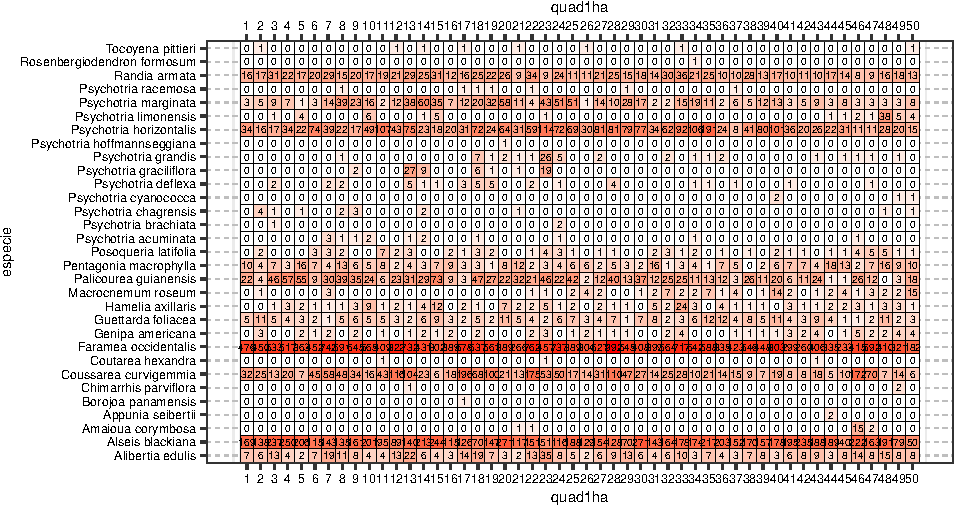
\includegraphics{manuscrito_files/figure-latex/unnamed-chunk-3-1.pdf}
\caption{\label{fig:abun_sp_q}Número de individuos de cada especie por
cuadrante.}
\end{figure}

\begin{figure}
\centering
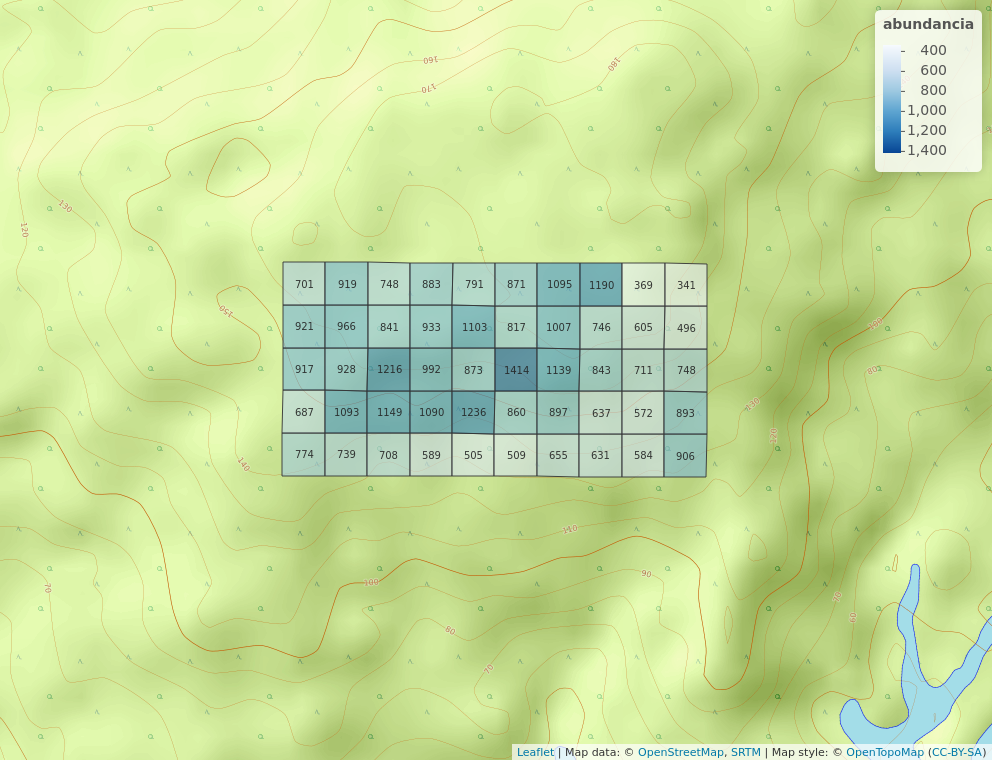
\includegraphics{mapa_cuadros_abun_rubic.png}
\caption{Abundancia de rubiaceas en BCI
\label{fig:mapa_cuadros_abun_rubic}}
\end{figure}

\begin{figure}
\centering
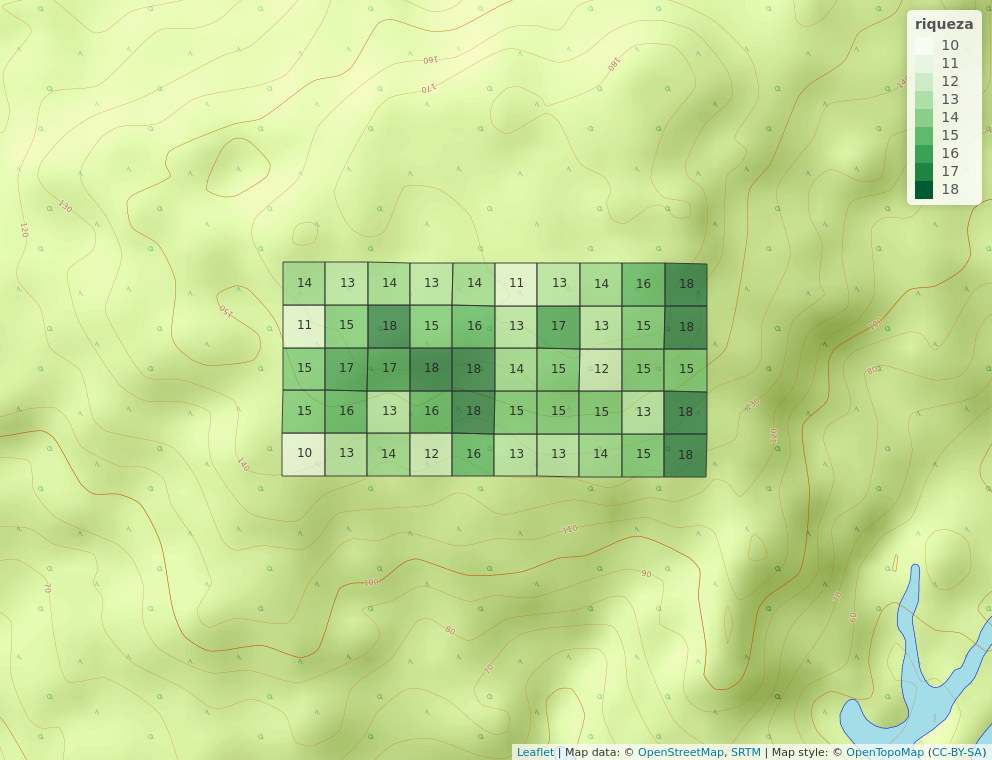
\includegraphics{mapa_cuadros_riq_rubic.png}
\caption{Distribución de la riqueza de rubiaceas en BCI
\label{fig:mapa_cuadros_riq}}
\end{figure}

\begin{figure}
\centering
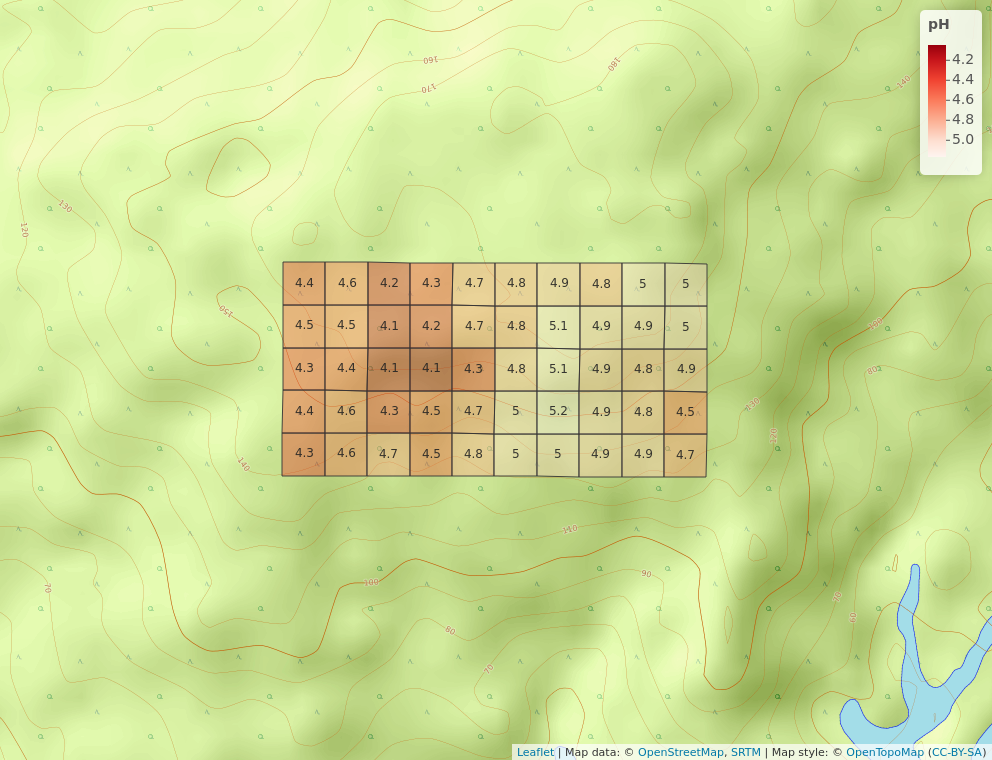
\includegraphics{mapa_cuadros_ph.png}
\caption{pH del suelo en los distintos cuadros de 1ha
\label{fig:mapa_cuadros_ph}}
\end{figure}

\section{Discusión}\label{discusiuxf3n}

Las variables cobre y fosforo en el suelo producieron una diferenciación
entre los grupos determinados. Se\\
Es importante que los analisis de agrupamiento pueden verse sesgados por
la heterogeneidad morfométrica que pueden presentar las plantas de esta
familia. Las especies de este grupo pueden presentar diversos hábitos de
crecimiento, que van desde el porte herbáceo y arbustivo a arboles
relativamente grandes. Esto hace que el hecho de que se incluya el
criterio de dap de 10 mm en el momento de ser censadas promueve a
alterar los datos, excluyendo especies de la comunidad de rubiaceas.

\section{Agradecimientos}\label{agradecimientos}

\section{Información de soporte}\label{informaciuxf3n-de-soporte}

\ldots

\section{\texorpdfstring{\emph{Script}
reproducible}{Script reproducible}}\label{script-reproducible}

\ldots

\section*{Referencias}\label{referencias}
\addcontentsline{toc}{section}{Referencias}

\hypertarget{refs}{}
\hypertarget{ref-cita_mapview}{}
Appelhans, T., Detsch, F., Reudenbach, C., \& Woellauer, S. (2019).
\emph{Mapview: Interactive viewing of spatial data in r}. Retrieved from
\url{https://CRAN.R-project.org/package=mapview}

\hypertarget{ref-borcard_legendre}{}
Borcard, D., Gillet, F., \& Legendre, P. (2018). \emph{Numerical Ecology
with R. Second Edition} (pp. 52--66).
\url{https://doi.org/10.1007/978-3-319-71404-2}

\hypertarget{ref-condit_et_al_2012}{}
Condit, R., Chisholm, R. A., \& Hubbell, S. P. (2012). Thirty years of
forest census at Barro Colorado and the importance of immigration in
maintaining diversity. \emph{PLOS ONE}, \emph{7}(11), 1--6.
\url{https://doi.org/10.1371/journal.pone.0049826}

\hypertarget{ref-condit_et_al_2017}{}
Condit, R., Pérez, R., Lao, S., Aguilar, S., \& Hubbell, S. P. (2017).
Demographic trends and climate over 35 years in the Barro Colorado 50 ha
plot. \emph{Forest Ecosystems}, \emph{4}(1), 17.
\url{https://doi.org/10.1186/s40663-017-0103-1}

\hypertarget{ref-article_condit}{}
Condit, R., Pitman, N., Leigh, E., Chave, J., Terborgh, J., Foster, R.,
\ldots{} Hubbell, S. (2002). Beta-diversity in tropical forest trees.
\emph{Science (New York, N.Y.)}, \emph{295}, 666--669.
\url{https://doi.org/10.1126/science.1066854}

\hypertarget{ref-davis2009global}{}
Davis, A. P., Govaerts, R., Bridson, D. M., Ruhsam, M., Moat, J., \&
Brummitt, N. A. (2009). A global assessment of distribution, diversity,
endemism, and taxonomic effort in the rubiaceae1. \emph{Annals of the
Missouri Botanical Garden}, \emph{96}(1), 68--78.

\hypertarget{ref-cita_indicspecies}{}
De Caceres, M., \& Legendre, P. (2009). Associations between species and
groups of sites: Indices and statistical inference. In \emph{Ecology}.
Retrieved from \url{http://sites.google.com/site/miqueldecaceres/}

\hypertarget{ref-dufrene_legendre}{}
Dufrene, M., \& Legendre, P. (1997). Species assemblages and indicator
species: The need for a flexible asymmetrical approach. \emph{Ecological
Monographs}, \emph{67}, 345--366. \url{https://doi.org/10.2307/2963459}

\hypertarget{ref-hubell_foster_1983}{}
Hubbell, S. P., \& Foster, R. B. (1983). Diversity of canopy trees in a
neotropical forest and implications for conservation. In T. Whitmore, A.
Chadwick, \& A. Sutton (Eds.), \emph{Tropical rain forest: Ecology and
management} (pp. 25--41). Oxford: The British Ecological Society.

\hypertarget{ref-hubell_et_all_1990}{}
Hubbell, S. P., Condit, R., Foster, R. B., Grubb, P. J., Thomas, C. D.,
Hassell, M. P., \& May, R. M. (1990). Presence and absence of density
dependence in a neotropical tree community. \emph{Philosophical
Transactions of the Royal Society of London. Series B: Biological
Sciences}, \emph{330}(1257), 269--281.
\url{https://doi.org/10.1098/rstb.1990.0198}

\hypertarget{ref-web_bci}{}
Hubbell, S., Condit, R., \& Foster, R. (2021). Forest Census Plot on
Barro Colorado Island. Retrieved March 23, 2021, from
\url{http://ctfs.si.edu/webatlas/datasets/bci/}

\hypertarget{ref-article}{}
Jansen, S., Robbrecht, E., Beeckman, H., \& Smets, E. (2000). Aluminium
accumulation in rubiaceae: An additional character for the delimitation
of the subfamily rubioideae? \emph{IAWA Journal}, \emph{21}.
\url{https://doi.org/10.1163/22941932-90000245}

\hypertarget{ref-legendre_galllagher_2001}{}
Legendre, P., \& Gallagher, E. (2001). Ecologically meaningful
transformations for ordination of species data. \emph{Oecologia},
\emph{129}, 271--280. \url{https://doi.org/10.1007/s004420100716}

\hypertarget{ref-jose_ramon_martinez_batlle_2020_4402362}{}
Martínez Batlle, J. R. (2020).
biogeografia-master/scripts-de-analisis-BCI: Long coding sessions
(Version v0.0.0.9000). \url{https://doi.org/10.5281/zenodo.4402362}

\hypertarget{ref-moreno2001manual}{}
Moreno, C. E. (2001). \emph{Manual de métodos para medir la
biodiversidad}. Universidad Veracruzana.

\hypertarget{ref-2008arXiv0803.3704N}{}
Néda, Z., Horvat, S., Toháti, H. M., Derzsi, A., \& Balogh, A. (2008). A
spatially explicit model for tropical tree diversity patterns.
\emph{arXiv E-Prints}, arXiv:0803.3704.

\hypertarget{ref-cita_vegan}{}
Oksanen, J., Blanchet, F. G., Friendly, M., Kindt, R., Legendre, P.,
McGlinn, D., \ldots{} Wagner, H. (2019). \emph{Vegan: Community ecology
package}. Retrieved from \url{https://CRAN.R-project.org/package=vegan}

\hypertarget{ref-cita_sf}{}
Pebesma, E. (2018). Simple Features for R: Standardized Support for
Spatial Vector Data. \emph{The R Journal}, \emph{10}(1), 439--446.
\url{https://doi.org/10.32614/RJ-2018-009}

\hypertarget{ref-cita_r}{}
R Core Team. (2020). \emph{R: A language and environment for statistical
computing}. Retrieved from \url{https://www.R-project.org/}

\hypertarget{ref-TORRESLEITE2019151487}{}
Torres-Leite, F., Cavatte, P. C., Garbin, M. L., Hollunder, R. K.,
Ferreira-Santos, K., Capetine, T. B., \ldots{} Carrijo, T. T. (2019).
Surviving in the shadows: Light responses of co-occurring rubiaceae
species within a tropical forest understory. \emph{Flora}, \emph{261},
151487.
\url{https://doi.org/https://doi.org/10.1016/j.flora.2019.151487}

\hypertarget{ref-Volkov_2003}{}
Volkov, I., Banavar, J. R., Hubbell, S. P., \& Maritan, A. (2003).
Neutral theory and relative species abundance in ecology. \emph{Nature},
\emph{424}(6952), 1035--1037. \url{https://doi.org/10.1038/nature01883}

\hypertarget{ref-cita_tidyverse}{}
Wickham, H. (2017). \emph{Tidyverse: Easily install and load the
'tidyverse'}. Retrieved from
\url{https://CRAN.R-project.org/package=tidyverse}




\newpage
\singlespacing 
\end{document}
